\documentclass{standalone}

\usepackage{tikz}

\begin{document}

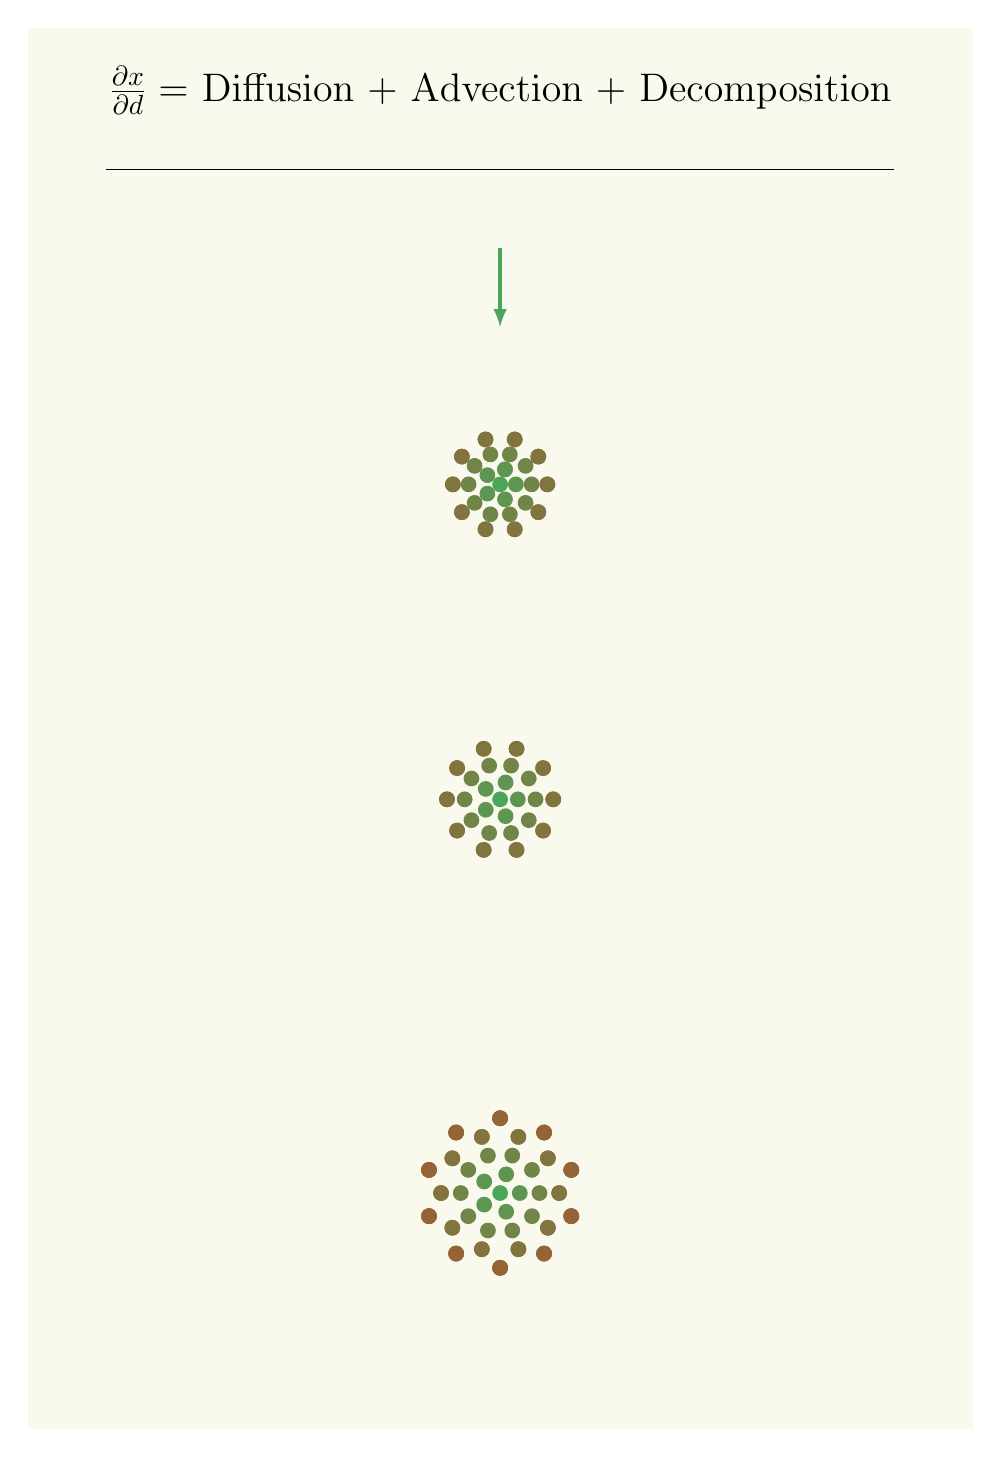
\begin{tikzpicture}
\fill[fill=gray!50!yellow!10] (-6,-18) rectangle (6,-0.2);

\draw (0,-1) node {\Large $\frac{\partial x}{\partial d} = $ Diffusion +  Advection + Decomposition};
%\draw (-4,-5) node {$Pe = 1$};
%\draw (4, -5) node {$\frac{\kappa}{v} = 1$};

\draw (-5,-2) -- (5,-2) ;
\draw[very thick, teal!70!yellow] [latex-] (0,-4) -- (0,-3) ;

\fill[teal!70!yellow] (0, -6) circle (0.1) ;
\foreach \x in{1,...,6}
\fill[teal!70!yellow!90!red] (0, -6) ++(\x *72:0.2) circle (0.1) ;

\foreach \x in{1,...,10}
\fill[teal!70!yellow!80!red] (0, -6) ++(\x * 36:0.4) circle (0.1) ;

\foreach \x in {1,...,20}
\fill[teal!70!yellow!70!red] (0, -6) ++(\x * 36:0.6) circle (0.1) ;

\fill[teal!70!yellow] (0, -10) circle (0.1) ;
\foreach \x in{1,...,5}
\fill[teal!70!yellow!90!red] (0, -10) ++(\x *72:0.225) circle (0.1) ;

\foreach \x in{1,...,10}
\fill[teal!70!yellow!80!red] (0, -10) ++(\x * 36:0.45) circle (0.1) ;

\foreach \x in {1,...,20}
\fill[teal!70!yellow!70!red] (0, -10) ++(\x * 36:0.675) circle (0.1) ;

\fill[teal!70!yellow] (0, -15) circle (0.1) ;
\foreach \x in{1,...,5}
\fill[teal!70!yellow!90!red] (0, -15) ++(\x *72:0.25) circle (0.1) ;

\foreach \x in{1,...,10}
\fill[teal!70!yellow!80!red] (0, -15) ++(\x * 36:0.5) circle (0.1) ;

\foreach \x in {1,...,20}
\fill[teal!70!yellow!70!red] (0, -15) ++(\x * 36:0.75) circle (0.1) ;

\foreach \x in{1,...,30}
\fill[teal!70!yellow!60!red] (0, -15) ++(\x *36+18:0.95) circle (0.1) ;

\end{tikzpicture}

% Created by tikzDevice version 0.12.4 on 2023-08-31 20:58:21
% !TEX encoding = UTF-8 Unicode
\documentclass[10pt]{article}
\usepackage{tikz}

\usepackage[active,tightpage,psfixbb]{preview}

\PreviewEnvironment{pgfpicture}

\setlength\PreviewBorder{0pt}
\begin{document}

\begin{tikzpicture}[x=1pt,y=1pt]
\definecolor{fillColor}{RGB}{255,255,255}
\path[use as bounding box,fill=fillColor,fill opacity=0.00] (0,0) rectangle (505.89,505.89);
\begin{scope}
\path[clip] ( 48.00, 48.00) rectangle (505.89,505.89);
\definecolor{drawColor}{RGB}{228,26,28}

\path[draw=drawColor,line width= 1.2pt,line join=round,line cap=round] (418.47,488.93) --
	(417.50,488.51) --
	(416.44,488.08) --
	(415.30,487.66) --
	(414.08,487.24) --
	(412.80,486.81) --
	(411.45,486.39) --
	(410.05,485.96) --
	(408.59,485.54) --
	(407.08,485.12) --
	(405.53,484.69) --
	(403.93,484.27) --
	(402.30,483.84) --
	(400.63,483.42) --
	(398.93,483.00) --
	(397.20,482.57) --
	(395.44,482.15) --
	(393.66,481.72) --
	(391.86,481.30) --
	(390.04,480.88) --
	(388.21,480.45) --
	(386.35,480.03) --
	(384.49,479.60) --
	(382.61,479.18) --
	(380.72,478.76) --
	(378.83,478.33) --
	(376.93,477.91) --
	(375.02,477.48) --
	(373.10,477.06) --
	(371.19,476.64) --
	(369.27,476.21) --
	(367.34,475.79) --
	(365.42,475.36) --
	(363.50,474.94) --
	(361.58,474.52) --
	(359.66,474.09) --
	(357.75,473.67) --
	(355.83,473.24) --
	(353.92,472.82) --
	(352.02,472.40) --
	(350.12,471.97) --
	(348.22,471.55) --
	(346.33,471.12) --
	(344.45,470.70) --
	(342.57,470.28) --
	(340.71,469.85) --
	(338.84,469.43) --
	(336.99,469.00) --
	(335.14,468.58) --
	(333.30,468.16) --
	(331.47,467.73) --
	(329.65,467.31) --
	(327.84,466.88) --
	(326.04,466.46) --
	(324.24,466.04) --
	(322.45,465.61) --
	(320.68,465.19) --
	(318.91,464.76) --
	(317.16,464.34) --
	(315.41,463.92) --
	(313.67,463.49) --
	(311.94,463.07) --
	(310.23,462.64) --
	(308.52,462.22) --
	(306.82,461.80) --
	(305.14,461.37) --
	(303.46,460.95) --
	(301.79,460.52) --
	(300.14,460.10) --
	(298.49,459.68) --
	(296.85,459.25) --
	(295.23,458.83) --
	(293.61,458.41) --
	(292.01,457.98) --
	(290.42,457.56) --
	(288.83,457.13) --
	(287.26,456.71) --
	(285.69,456.29) --
	(284.14,455.86) --
	(282.60,455.44) --
	(281.06,455.01) --
	(279.54,454.59) --
	(278.03,454.17) --
	(276.53,453.74) --
	(275.03,453.32) --
	(273.55,452.89) --
	(272.08,452.47) --
	(270.62,452.05) --
	(269.17,451.62) --
	(267.72,451.20) --
	(266.29,450.77) --
	(264.87,450.35) --
	(263.45,449.93) --
	(262.05,449.50) --
	(260.66,449.08) --
	(259.27,448.65) --
	(257.90,448.23) --
	(256.53,447.81) --
	(255.18,447.38) --
	(253.83,446.96) --
	(252.49,446.53) --
	(251.17,446.11) --
	(249.85,445.69) --
	(248.54,445.26) --
	(247.24,444.84) --
	(245.95,444.41) --
	(244.67,443.99) --
	(243.39,443.57) --
	(242.13,443.14) --
	(240.87,442.72) --
	(239.63,442.29) --
	(238.39,441.87) --
	(237.16,441.45) --
	(235.94,441.02) --
	(234.73,440.60) --
	(233.53,440.17) --
	(232.33,439.75) --
	(231.14,439.33) --
	(229.97,438.90) --
	(228.80,438.48) --
	(227.63,438.05) --
	(226.48,437.63) --
	(225.34,437.21) --
	(224.20,436.78) --
	(223.07,436.36) --
	(221.95,435.93) --
	(220.84,435.51) --
	(219.73,435.09) --
	(218.63,434.66) --
	(217.54,434.24) --
	(216.46,433.81) --
	(215.39,433.39) --
	(214.32,432.97) --
	(213.26,432.54) --
	(212.21,432.12) --
	(211.16,431.69) --
	(210.13,431.27) --
	(209.10,430.85) --
	(208.08,430.42) --
	(207.06,430.00) --
	(206.05,429.57) --
	(205.05,429.15) --
	(204.06,428.73) --
	(203.07,428.30) --
	(202.09,427.88) --
	(201.12,427.46) --
	(200.15,427.03) --
	(199.20,426.61) --
	(198.24,426.18) --
	(197.30,425.76) --
	(196.36,425.34) --
	(195.43,424.91) --
	(194.50,424.49) --
	(193.58,424.06) --
	(192.67,423.64) --
	(191.77,423.22) --
	(190.87,422.79) --
	(189.97,422.37) --
	(189.09,421.94) --
	(188.21,421.52) --
	(187.33,421.10) --
	(186.47,420.67) --
	(185.60,420.25) --
	(184.75,419.82) --
	(183.90,419.40) --
	(183.06,418.98) --
	(182.22,418.55) --
	(181.39,418.13) --
	(180.56,417.70) --
	(179.74,417.28) --
	(178.93,416.86) --
	(178.12,416.43) --
	(177.32,416.01) --
	(176.52,415.58) --
	(175.73,415.16) --
	(174.94,414.74) --
	(174.16,414.31) --
	(173.39,413.89) --
	(172.62,413.46) --
	(171.86,413.04) --
	(171.10,412.62) --
	(170.35,412.19) --
	(169.60,411.77) --
	(168.86,411.34) --
	(168.12,410.92) --
	(167.39,410.50) --
	(166.67,410.07) --
	(165.94,409.65) --
	(165.23,409.22) --
	(164.52,408.80) --
	(163.81,408.38) --
	(163.11,407.95) --
	(162.42,407.53) --
	(161.72,407.10) --
	(161.04,406.68) --
	(160.36,406.26) --
	(159.68,405.83) --
	(159.01,405.41) --
	(158.34,404.98) --
	(157.68,404.56) --
	(157.02,404.14) --
	(156.37,403.71) --
	(155.72,403.29) --
	(155.08,402.86) --
	(154.44,402.44) --
	(153.81,402.02) --
	(153.18,401.59) --
	(152.55,401.17) --
	(151.93,400.74) --
	(151.32,400.32) --
	(150.71,399.90) --
	(150.10,399.47) --
	(149.49,399.05) --
	(148.90,398.63) --
	(148.30,398.20) --
	(147.71,397.78) --
	(147.12,397.35) --
	(146.54,396.93) --
	(145.96,396.51) --
	(145.39,396.08) --
	(144.82,395.66) --
	(144.25,395.23) --
	(143.69,394.81) --
	(143.13,394.39) --
	(142.58,393.96) --
	(142.03,393.54) --
	(141.49,393.11) --
	(140.94,392.69) --
	(140.40,392.27) --
	(139.87,391.84) --
	(139.34,391.42) --
	(138.81,390.99) --
	(138.29,390.57) --
	(137.77,390.15) --
	(137.25,389.72) --
	(136.74,389.30) --
	(136.23,388.87) --
	(135.73,388.45) --
	(135.23,388.03) --
	(134.73,387.60) --
	(134.24,387.18) --
	(133.75,386.75) --
	(133.26,386.33) --
	(132.78,385.91) --
	(132.30,385.48) --
	(131.82,385.06) --
	(131.35,384.63) --
	(130.88,384.21) --
	(130.41,383.79) --
	(129.94,383.36) --
	(129.48,382.94) --
	(129.03,382.51) --
	(128.57,382.09) --
	(128.12,381.67) --
	(127.68,381.24) --
	(127.23,380.82) --
	(126.79,380.39) --
	(126.35,379.97) --
	(125.92,379.55) --
	(125.49,379.12) --
	(125.06,378.70) --
	(124.63,378.27) --
	(124.21,377.85) --
	(123.79,377.43) --
	(123.38,377.00) --
	(122.96,376.58) --
	(122.55,376.15) --
	(122.14,375.73) --
	(121.74,375.31) --
	(121.34,374.88) --
	(120.94,374.46) --
	(120.54,374.03) --
	(120.15,373.61) --
	(119.76,373.19) --
	(119.37,372.76) --
	(118.99,372.34) --
	(118.60,371.91) --
	(118.22,371.49) --
	(117.85,371.07) --
	(117.47,370.64) --
	(117.10,370.22) --
	(116.73,369.79) --
	(116.37,369.37) --
	(116.00,368.95) --
	(115.64,368.52) --
	(115.28,368.10) --
	(114.93,367.68) --
	(114.57,367.25) --
	(114.22,366.83) --
	(113.87,366.40) --
	(113.53,365.98) --
	(113.18,365.56) --
	(112.84,365.13) --
	(112.50,364.71) --
	(112.17,364.28) --
	(111.83,363.86) --
	(111.50,363.44) --
	(111.17,363.01) --
	(110.85,362.59) --
	(110.52,362.16) --
	(110.20,361.74) --
	(109.88,361.32) --
	(109.56,360.89) --
	(109.25,360.47) --
	(108.93,360.04) --
	(108.62,359.62) --
	(108.31,359.20) --
	(108.01,358.77) --
	(107.70,358.35) --
	(107.40,357.92) --
	(107.10,357.50) --
	(106.80,357.08) --
	(106.51,356.65) --
	(106.21,356.23) --
	(105.92,355.80) --
	(105.63,355.38) --
	(105.34,354.96) --
	(105.06,354.53) --
	(104.77,354.11) --
	(104.49,353.68) --
	(104.21,353.26) --
	(103.94,352.84) --
	(103.66,352.41) --
	(103.39,351.99) --
	(103.11,351.56) --
	(102.85,351.14) --
	(102.58,350.72) --
	(102.31,350.29) --
	(102.05,349.87) --
	(101.79,349.44) --
	(101.52,349.02) --
	(101.27,348.60) --
	(101.01,348.17) --
	(100.76,347.75) --
	(100.50,347.32) --
	(100.25,346.90) --
	(100.00,346.48) --
	( 99.75,346.05) --
	( 99.51,345.63) --
	( 99.26,345.20) --
	( 99.02,344.78) --
	( 98.78,344.36) --
	( 98.54,343.93) --
	( 98.30,343.51) --
	( 98.07,343.08) --
	( 97.83,342.66) --
	( 97.60,342.24) --
	( 97.37,341.81) --
	( 97.14,341.39) --
	( 96.92,340.96) --
	( 96.69,340.54) --
	( 96.47,340.12) --
	( 96.24,339.69) --
	( 96.02,339.27) --
	( 95.80,338.84) --
	( 95.58,338.42) --
	( 95.37,338.00) --
	( 95.15,337.57) --
	( 94.94,337.15) --
	( 94.73,336.73) --
	( 94.52,336.30) --
	( 94.31,335.88) --
	( 94.10,335.45) --
	( 93.90,335.03) --
	( 93.69,334.61) --
	( 93.49,334.18) --
	( 93.29,333.76) --
	( 93.09,333.33) --
	( 92.89,332.91) --
	( 92.69,332.49) --
	( 92.50,332.06) --
	( 92.30,331.64) --
	( 92.11,331.21) --
	( 91.92,330.79) --
	( 91.73,330.37) --
	( 91.54,329.94) --
	( 91.35,329.52) --
	( 91.16,329.09) --
	( 90.98,328.67) --
	( 90.79,328.25) --
	( 90.61,327.82) --
	( 90.43,327.40) --
	( 90.25,326.97) --
	( 90.07,326.55) --
	( 89.90,326.13) --
	( 89.72,325.70) --
	( 89.54,325.28) --
	( 89.37,324.85) --
	( 89.20,324.43) --
	( 89.03,324.01) --
	( 88.86,323.58) --
	( 88.69,323.16) --
	( 88.52,322.73) --
	( 88.36,322.31) --
	( 88.19,321.89) --
	( 88.03,321.46) --
	( 87.86,321.04) --
	( 87.70,320.61) --
	( 87.54,320.19) --
	( 87.38,319.77) --
	( 87.22,319.34) --
	( 87.07,318.92) --
	( 86.91,318.49) --
	( 86.76,318.07) --
	( 86.60,317.65) --
	( 86.45,317.22) --
	( 86.30,316.80) --
	( 86.15,316.37) --
	( 86.00,315.95) --
	( 85.85,315.53) --
	( 85.70,315.10) --
	( 85.56,314.68) --
	( 85.41,314.25) --
	( 85.27,313.83) --
	( 85.12,313.41) --
	( 84.98,312.98) --
	( 84.84,312.56) --
	( 84.70,312.13) --
	( 84.56,311.71) --
	( 84.42,311.29) --
	( 84.28,310.86) --
	( 84.15,310.44) --
	( 84.01,310.01) --
	( 83.88,309.59) --
	( 83.74,309.17) --
	( 83.61,308.74) --
	( 83.48,308.32) --
	( 83.35,307.89) --
	( 83.22,307.47) --
	( 83.09,307.05) --
	( 82.96,306.62) --
	( 82.84,306.20) --
	( 82.71,305.78) --
	( 82.59,305.35) --
	( 82.46,304.93) --
	( 82.34,304.50) --
	( 82.22,304.08) --
	( 82.09,303.66) --
	( 81.97,303.23) --
	( 81.85,302.81) --
	( 81.73,302.38) --
	( 81.62,301.96) --
	( 81.50,301.54) --
	( 81.38,301.11) --
	( 81.27,300.69) --
	( 81.15,300.26) --
	( 81.04,299.84) --
	( 80.92,299.42) --
	( 80.81,298.99) --
	( 80.70,298.57) --
	( 80.59,298.14) --
	( 80.48,297.72) --
	( 80.37,297.30) --
	( 80.26,296.87) --
	( 80.15,296.45) --
	( 80.05,296.02) --
	( 79.94,295.60) --
	( 79.83,295.18) --
	( 79.73,294.75) --
	( 79.62,294.33) --
	( 79.52,293.90) --
	( 79.42,293.48) --
	( 79.32,293.06) --
	( 79.22,292.63) --
	( 79.12,292.21) --
	( 79.02,291.78) --
	( 78.92,291.36) --
	( 78.82,290.94) --
	( 78.72,290.51) --
	( 78.62,290.09) --
	( 78.53,289.66) --
	( 78.43,289.24) --
	( 78.34,288.82) --
	( 78.24,288.39) --
	( 78.15,287.97) --
	( 78.06,287.54) --
	( 77.96,287.12) --
	( 77.87,286.70) --
	( 77.78,286.27) --
	( 77.69,285.85) --
	( 77.60,285.42) --
	( 77.51,285.00) --
	( 77.42,284.58) --
	( 77.34,284.15) --
	( 77.25,283.73) --
	( 77.16,283.30) --
	( 77.08,282.88) --
	( 76.99,282.46) --
	( 76.91,282.03) --
	( 76.82,281.61) --
	( 76.74,281.18) --
	( 76.66,280.76) --
	( 76.57,280.34) --
	( 76.49,279.91) --
	( 76.41,279.49) --
	( 76.33,279.06) --
	( 76.25,278.64) --
	( 76.17,278.22) --
	( 76.09,277.79) --
	( 76.01,277.37) --
	( 75.94,276.94) --
	( 75.86,276.52) --
	( 75.78,276.10) --
	( 75.71,275.67) --
	( 75.63,275.25) --
	( 75.55,274.83) --
	( 75.48,274.40) --
	( 75.41,273.98) --
	( 75.33,273.55) --
	( 75.26,273.13) --
	( 75.19,272.71) --
	( 75.12,272.28) --
	( 75.04,271.86) --
	( 74.97,271.43) --
	( 74.90,271.01) --
	( 74.83,270.59) --
	( 74.76,270.16) --
	( 74.69,269.74) --
	( 74.63,269.31) --
	( 74.56,268.89) --
	( 74.49,268.47) --
	( 74.42,268.04) --
	( 74.36,267.62) --
	( 74.29,267.19) --
	( 74.22,266.77) --
	( 74.16,266.35) --
	( 74.09,265.92) --
	( 74.03,265.50) --
	( 73.97,265.07) --
	( 73.90,264.65) --
	( 73.84,264.23) --
	( 73.78,263.80) --
	( 73.72,263.38) --
	( 73.65,262.95) --
	( 73.59,262.53) --
	( 73.53,262.11) --
	( 73.47,261.68) --
	( 73.41,261.26) --
	( 73.35,260.83) --
	( 73.29,260.41) --
	( 73.24,259.99) --
	( 73.18,259.56) --
	( 73.12,259.14) --
	( 73.06,258.71) --
	( 73.01,258.29) --
	( 72.95,257.87) --
	( 72.89,257.44) --
	( 72.84,257.02) --
	( 72.78,256.59) --
	( 72.73,256.17) --
	( 72.67,255.75) --
	( 72.62,255.32) --
	( 72.56,254.90) --
	( 72.51,254.47) --
	( 72.46,254.05) --
	( 72.40,253.63) --
	( 72.35,253.20) --
	( 72.30,252.78) --
	( 72.25,252.35) --
	( 72.20,251.93) --
	( 72.15,251.51) --
	( 72.10,251.08) --
	( 72.05,250.66) --
	( 72.00,250.23) --
	( 71.95,249.81) --
	( 71.90,249.39) --
	( 71.85,248.96) --
	( 71.80,248.54) --
	( 71.75,248.11) --
	( 71.70,247.69) --
	( 71.66,247.27) --
	( 71.61,246.84) --
	( 71.56,246.42) --
	( 71.52,246.00) --
	( 71.47,245.57) --
	( 71.43,245.15) --
	( 71.38,244.72) --
	( 71.33,244.30) --
	( 71.29,243.88) --
	( 71.25,243.45) --
	( 71.20,243.03) --
	( 71.16,242.60) --
	( 71.11,242.18) --
	( 71.07,241.76) --
	( 71.03,241.33) --
	( 70.99,240.91) --
	( 70.94,240.48) --
	( 70.90,240.06) --
	( 70.86,239.64) --
	( 70.82,239.21) --
	( 70.78,238.79) --
	( 70.74,238.36) --
	( 70.70,237.94) --
	( 70.66,237.52) --
	( 70.62,237.09) --
	( 70.58,236.67) --
	( 70.54,236.24) --
	( 70.50,235.82) --
	( 70.46,235.40) --
	( 70.42,234.97) --
	( 70.38,234.55) --
	( 70.34,234.12) --
	( 70.31,233.70) --
	( 70.27,233.28) --
	( 70.23,232.85) --
	( 70.19,232.43) --
	( 70.16,232.00) --
	( 70.12,231.58) --
	( 70.08,231.16) --
	( 70.05,230.73) --
	( 70.01,230.31) --
	( 69.98,229.88) --
	( 69.94,229.46) --
	( 69.91,229.04) --
	( 69.87,228.61) --
	( 69.84,228.19) --
	( 69.80,227.76) --
	( 69.77,227.34) --
	( 69.74,226.92) --
	( 69.70,226.49) --
	( 69.67,226.07) --
	( 69.64,225.64) --
	( 69.60,225.22) --
	( 69.57,224.80) --
	( 69.54,224.37) --
	( 69.51,223.95) --
	( 69.47,223.52) --
	( 69.44,223.10) --
	( 69.41,222.68) --
	( 69.38,222.25) --
	( 69.35,221.83) --
	( 69.32,221.40) --
	( 69.29,220.98) --
	( 69.26,220.56) --
	( 69.23,220.13) --
	( 69.20,219.71) --
	( 69.17,219.28) --
	( 69.14,218.86) --
	( 69.11,218.44) --
	( 69.08,218.01) --
	( 69.05,217.59) --
	( 69.02,217.16) --
	( 68.99,216.74) --
	( 68.97,216.32) --
	( 68.94,215.89) --
	( 68.91,215.47) --
	( 68.88,215.05) --
	( 68.85,214.62) --
	( 68.83,214.20) --
	( 68.80,213.77) --
	( 68.77,213.35) --
	( 68.75,212.93) --
	( 68.72,212.50) --
	( 68.69,212.08) --
	( 68.67,211.65) --
	( 68.64,211.23) --
	( 68.62,210.81) --
	( 68.59,210.38) --
	( 68.56,209.96) --
	( 68.54,209.53) --
	( 68.51,209.11) --
	( 68.49,208.69) --
	( 68.46,208.26) --
	( 68.44,207.84) --
	( 68.42,207.41) --
	( 68.39,206.99) --
	( 68.37,206.57) --
	( 68.34,206.14) --
	( 68.32,205.72) --
	( 68.30,205.29) --
	( 68.27,204.87) --
	( 68.25,204.45) --
	( 68.23,204.02) --
	( 68.20,203.60) --
	( 68.18,203.17) --
	( 68.16,202.75) --
	( 68.14,202.33) --
	( 68.11,201.90) --
	( 68.09,201.48) --
	( 68.07,201.05) --
	( 68.05,200.63) --
	( 68.03,200.21) --
	( 68.01,199.78) --
	( 67.98,199.36) --
	( 67.96,198.93) --
	( 67.94,198.51) --
	( 67.92,198.09) --
	( 67.90,197.66) --
	( 67.88,197.24) --
	( 67.86,196.81) --
	( 67.84,196.39) --
	( 67.82,195.97) --
	( 67.80,195.54) --
	( 67.78,195.12) --
	( 67.76,194.69) --
	( 67.74,194.27) --
	( 67.72,193.85) --
	( 67.70,193.42) --
	( 67.68,193.00) --
	( 67.66,192.57) --
	( 67.64,192.15) --
	( 67.62,191.73) --
	( 67.61,191.30) --
	( 67.59,190.88) --
	( 67.57,190.45) --
	( 67.55,190.03) --
	( 67.53,189.61) --
	( 67.51,189.18) --
	( 67.50,188.76) --
	( 67.48,188.33) --
	( 67.46,187.91) --
	( 67.44,187.49) --
	( 67.43,187.06) --
	( 67.41,186.64) --
	( 67.39,186.21) --
	( 67.38,185.79) --
	( 67.36,185.37) --
	( 67.34,184.94) --
	( 67.33,184.52) --
	( 67.31,184.10) --
	( 67.29,183.67) --
	( 67.28,183.25) --
	( 67.26,182.82) --
	( 67.24,182.40) --
	( 67.23,181.98) --
	( 67.21,181.55) --
	( 67.20,181.13) --
	( 67.18,180.70) --
	( 67.16,180.28) --
	( 67.15,179.86) --
	( 67.13,179.43) --
	( 67.12,179.01) --
	( 67.10,178.58) --
	( 67.09,178.16) --
	( 67.07,177.74) --
	( 67.06,177.31) --
	( 67.04,176.89) --
	( 67.03,176.46) --
	( 67.02,176.04) --
	( 67.00,175.62) --
	( 66.99,175.19) --
	( 66.97,174.77) --
	( 66.96,174.34) --
	( 66.94,173.92) --
	( 66.93,173.50) --
	( 66.92,173.07) --
	( 66.90,172.65) --
	( 66.89,172.22) --
	( 66.88,171.80) --
	( 66.86,171.38) --
	( 66.85,170.95) --
	( 66.84,170.53) --
	( 66.82,170.10) --
	( 66.81,169.68) --
	( 66.80,169.26) --
	( 66.78,168.83) --
	( 66.77,168.41) --
	( 66.76,167.98) --
	( 66.75,167.56) --
	( 66.73,167.14) --
	( 66.72,166.71) --
	( 66.71,166.29) --
	( 66.70,165.86) --
	( 66.69,165.44) --
	( 66.67,165.02) --
	( 66.66,164.59) --
	( 66.65,164.17) --
	( 66.64,163.74) --
	( 66.63,163.32) --
	( 66.61,162.90) --
	( 66.60,162.47) --
	( 66.59,162.05) --
	( 66.58,161.62) --
	( 66.57,161.20) --
	( 66.56,160.78) --
	( 66.55,160.35) --
	( 66.54,159.93) --
	( 66.52,159.50) --
	( 66.51,159.08) --
	( 66.50,158.66) --
	( 66.49,158.23) --
	( 66.48,157.81) --
	( 66.47,157.38) --
	( 66.46,156.96) --
	( 66.45,156.54) --
	( 66.44,156.11) --
	( 66.43,155.69) --
	( 66.42,155.26) --
	( 66.41,154.84) --
	( 66.40,154.42) --
	( 66.39,153.99) --
	( 66.38,153.57) --
	( 66.37,153.15) --
	( 66.36,152.72) --
	( 66.35,152.30) --
	( 66.34,151.87) --
	( 66.33,151.45) --
	( 66.32,151.03) --
	( 66.31,150.60) --
	( 66.30,150.18) --
	( 66.29,149.75) --
	( 66.28,149.33) --
	( 66.27,148.91) --
	( 66.26,148.48) --
	( 66.25,148.06) --
	( 66.25,147.63) --
	( 66.24,147.21) --
	( 66.23,146.79) --
	( 66.22,146.36) --
	( 66.21,145.94) --
	( 66.20,145.51) --
	( 66.19,145.09) --
	( 66.18,144.67) --
	( 66.18,144.24) --
	( 66.17,143.82) --
	( 66.16,143.39) --
	( 66.15,142.97) --
	( 66.14,142.55) --
	( 66.13,142.12) --
	( 66.13,141.70) --
	( 66.12,141.27) --
	( 66.11,140.85) --
	( 66.10,140.43) --
	( 66.09,140.00) --
	( 66.09,139.58) --
	( 66.08,139.15) --
	( 66.07,138.73) --
	( 66.06,138.31) --
	( 66.05,137.88) --
	( 66.05,137.46) --
	( 66.04,137.03) --
	( 66.03,136.61) --
	( 66.02,136.19) --
	( 66.02,135.76) --
	( 66.01,135.34) --
	( 66.00,134.91) --
	( 66.00,134.49) --
	( 65.99,134.07) --
	( 65.98,133.64) --
	( 65.97,133.22) --
	( 65.97,132.79) --
	( 65.96,132.37) --
	( 65.95,131.95) --
	( 65.95,131.52) --
	( 65.94,131.10) --
	( 65.93,130.67) --
	( 65.93,130.25) --
	( 65.92,129.83) --
	( 65.91,129.40) --
	( 65.91,128.98) --
	( 65.90,128.55) --
	( 65.89,128.13) --
	( 65.89,127.71) --
	( 65.88,127.28) --
	( 65.87,126.86) --
	( 65.87,126.43) --
	( 65.86,126.01) --
	( 65.85,125.59) --
	( 65.85,125.16) --
	( 65.84,124.74) --
	( 65.84,124.31) --
	( 65.83,123.89) --
	( 65.82,123.47) --
	( 65.82,123.04) --
	( 65.81,122.62) --
	( 65.81,122.20) --
	( 65.80,121.77) --
	( 65.79,121.35) --
	( 65.79,120.92) --
	( 65.78,120.50) --
	( 65.78,120.08) --
	( 65.77,119.65) --
	( 65.77,119.23) --
	( 65.76,118.80) --
	( 65.75,118.38) --
	( 65.75,117.96) --
	( 65.74,117.53) --
	( 65.74,117.11) --
	( 65.73,116.68) --
	( 65.73,116.26) --
	( 65.72,115.84) --
	( 65.72,115.41) --
	( 65.71,114.99) --
	( 65.71,114.56) --
	( 65.70,114.14) --
	( 65.70,113.72) --
	( 65.69,113.29) --
	( 65.69,112.87) --
	( 65.68,112.44) --
	( 65.68,112.02) --
	( 65.67,111.60) --
	( 65.67,111.17) --
	( 65.66,110.75) --
	( 65.66,110.32) --
	( 65.65,109.90) --
	( 65.65,109.48) --
	( 65.64,109.05) --
	( 65.64,108.63) --
	( 65.63,108.20) --
	( 65.63,107.78) --
	( 65.62,107.36) --
	( 65.62,106.93) --
	( 65.61,106.51) --
	( 65.61,106.08) --
	( 65.60,105.66) --
	( 65.60,105.24) --
	( 65.60,104.81) --
	( 65.59,104.39) --
	( 65.59,103.96) --
	( 65.58,103.54) --
	( 65.58,103.12) --
	( 65.57,102.69) --
	( 65.57,102.27) --
	( 65.56,101.84) --
	( 65.56,101.42) --
	( 65.56,101.00) --
	( 65.55,100.57) --
	( 65.55,100.15) --
	( 65.54, 99.72) --
	( 65.54, 99.30) --
	( 65.54, 98.88) --
	( 65.53, 98.45) --
	( 65.53, 98.03) --
	( 65.52, 97.60) --
	( 65.52, 97.18) --
	( 65.52, 96.76) --
	( 65.51, 96.33) --
	( 65.51, 95.91) --
	( 65.50, 95.48) --
	( 65.50, 95.06) --
	( 65.50, 94.64) --
	( 65.49, 94.21) --
	( 65.49, 93.79) --
	( 65.49, 93.37) --
	( 65.48, 92.94) --
	( 65.48, 92.52) --
	( 65.48, 92.09) --
	( 65.47, 91.67) --
	( 65.47, 91.25) --
	( 65.46, 90.82) --
	( 65.46, 90.40) --
	( 65.46, 89.97) --
	( 65.45, 89.55) --
	( 65.45, 89.13) --
	( 65.45, 88.70) --
	( 65.44, 88.28) --
	( 65.44, 87.85) --
	( 65.44, 87.43) --
	( 65.43, 87.01) --
	( 65.43, 86.58) --
	( 65.43, 86.16) --
	( 65.42, 85.73) --
	( 65.42, 85.31) --
	( 65.42, 84.89) --
	( 65.41, 84.46) --
	( 65.41, 84.04) --
	( 65.41, 83.61) --
	( 65.40, 83.19) --
	( 65.40, 82.77) --
	( 65.40, 82.34) --
	( 65.39, 81.92) --
	( 65.39, 81.49) --
	( 65.39, 81.07) --
	( 65.38, 80.65) --
	( 65.38, 80.22) --
	( 65.38, 79.80) --
	( 65.37, 79.37) --
	( 65.37, 78.95) --
	( 65.37, 78.53) --
	( 65.36, 78.10) --
	( 65.36, 77.68) --
	( 65.36, 77.25) --
	( 65.35, 76.83) --
	( 65.35, 76.41) --
	( 65.34, 75.98) --
	( 65.34, 75.56) --
	( 65.33, 75.13) --
	( 65.33, 74.71) --
	( 65.32, 74.29) --
	( 65.32, 73.86) --
	( 65.31, 73.44) --
	( 65.31, 73.01) --
	( 65.30, 72.59) --
	( 65.29, 72.17) --
	( 65.29, 71.74) --
	( 65.28, 71.32) --
	( 65.27, 70.89) --
	( 65.26, 70.47) --
	( 65.25, 70.05) --
	( 65.23, 69.62) --
	( 65.22, 69.20) --
	( 65.21, 68.77) --
	( 65.19, 68.35) --
	( 65.17, 67.93) --
	( 65.15, 67.50) --
	( 65.13, 67.08) --
	( 65.10, 66.65) --
	( 65.07, 66.23) --
	( 65.04, 65.81) --
	( 65.00, 65.38) --
	( 64.96, 64.96);
\end{scope}
\begin{scope}
\path[clip] (  0.00,  0.00) rectangle (505.89,505.89);
\definecolor{drawColor}{RGB}{0,0,0}

\path[draw=drawColor,line width= 0.4pt,line join=round,line cap=round] ( 64.96, 48.00) -- (488.93, 48.00);

\path[draw=drawColor,line width= 0.4pt,line join=round,line cap=round] ( 64.96, 48.00) -- ( 64.96, 42.00);

\path[draw=drawColor,line width= 0.4pt,line join=round,line cap=round] (149.75, 48.00) -- (149.75, 42.00);

\path[draw=drawColor,line width= 0.4pt,line join=round,line cap=round] (234.55, 48.00) -- (234.55, 42.00);

\path[draw=drawColor,line width= 0.4pt,line join=round,line cap=round] (319.34, 48.00) -- (319.34, 42.00);

\path[draw=drawColor,line width= 0.4pt,line join=round,line cap=round] (404.14, 48.00) -- (404.14, 42.00);

\path[draw=drawColor,line width= 0.4pt,line join=round,line cap=round] (488.93, 48.00) -- (488.93, 42.00);

\node[text=drawColor,anchor=base,inner sep=0pt, outer sep=0pt, scale=  1.00] at ( 64.96, 26.40) {0.00};

\node[text=drawColor,anchor=base,inner sep=0pt, outer sep=0pt, scale=  1.00] at (149.75, 26.40) {0.02};

\node[text=drawColor,anchor=base,inner sep=0pt, outer sep=0pt, scale=  1.00] at (234.55, 26.40) {0.04};

\node[text=drawColor,anchor=base,inner sep=0pt, outer sep=0pt, scale=  1.00] at (319.34, 26.40) {0.06};

\node[text=drawColor,anchor=base,inner sep=0pt, outer sep=0pt, scale=  1.00] at (404.14, 26.40) {0.08};

\node[text=drawColor,anchor=base,inner sep=0pt, outer sep=0pt, scale=  1.00] at (488.93, 26.40) {0.10};
\end{scope}
\begin{scope}
\path[clip] (  0.00,  0.00) rectangle (505.89,505.89);
\definecolor{drawColor}{RGB}{0,0,0}

\node[text=drawColor,anchor=base west,inner sep=0pt, outer sep=0pt, scale=  1.00] at (223.06,  4.90) {C concentration (g c};

\node[text=drawColor,anchor=base west,inner sep=0pt, outer sep=0pt, scale=  1.00] at (312.78,  4.90) {m};

\node[text=drawColor,anchor=base west,inner sep=0pt, outer sep=0pt, scale=  0.70] at (321.11,  8.99) {-};

\node[text=drawColor,anchor=base west,inner sep=0pt, outer sep=0pt, scale=  0.70] at (323.45,  8.99) {3};

\node[text=drawColor,anchor=base west,inner sep=0pt, outer sep=0pt, scale=  1.00] at (326.95,  4.90) {)};

\node[text=drawColor,rotate= 90.00,anchor=base,inner sep=0pt, outer sep=0pt, scale=  1.00] at (  9.60,276.94) {Depth (cm)};
\end{scope}
\begin{scope}
\path[clip] (  0.00,  0.00) rectangle (505.89,505.89);
\definecolor{drawColor}{RGB}{0,0,0}

\path[draw=drawColor,line width= 0.4pt,line join=round,line cap=round] ( 48.00, 64.96) -- ( 48.00,488.93);

\path[draw=drawColor,line width= 0.4pt,line join=round,line cap=round] ( 48.00, 64.96) -- ( 42.00, 64.96);

\path[draw=drawColor,line width= 0.4pt,line join=round,line cap=round] ( 48.00,149.75) -- ( 42.00,149.75);

\path[draw=drawColor,line width= 0.4pt,line join=round,line cap=round] ( 48.00,234.55) -- ( 42.00,234.55);

\path[draw=drawColor,line width= 0.4pt,line join=round,line cap=round] ( 48.00,319.34) -- ( 42.00,319.34);

\path[draw=drawColor,line width= 0.4pt,line join=round,line cap=round] ( 48.00,404.14) -- ( 42.00,404.14);

\path[draw=drawColor,line width= 0.4pt,line join=round,line cap=round] ( 48.00,488.93) -- ( 42.00,488.93);

\node[text=drawColor,rotate= 90.00,anchor=base,inner sep=0pt, outer sep=0pt, scale=  1.00] at ( 33.60, 64.96) {100};

\node[text=drawColor,rotate= 90.00,anchor=base,inner sep=0pt, outer sep=0pt, scale=  1.00] at ( 33.60,149.75) {80};

\node[text=drawColor,rotate= 90.00,anchor=base,inner sep=0pt, outer sep=0pt, scale=  1.00] at ( 33.60,234.55) {60};

\node[text=drawColor,rotate= 90.00,anchor=base,inner sep=0pt, outer sep=0pt, scale=  1.00] at ( 33.60,319.34) {40};

\node[text=drawColor,rotate= 90.00,anchor=base,inner sep=0pt, outer sep=0pt, scale=  1.00] at ( 33.60,404.14) {20};

\node[text=drawColor,rotate= 90.00,anchor=base,inner sep=0pt, outer sep=0pt, scale=  1.00] at ( 33.60,488.93) {0};
\end{scope}
\begin{scope}
\path[clip] ( 48.00, 48.00) rectangle (505.89,505.89);
\definecolor{drawColor}{RGB}{55,126,184}

\path[draw=drawColor,line width= 1.2pt,line join=round,line cap=round] (418.47,488.93) --
	(418.47,488.51) --
	(418.47,488.08) --
	(418.46,487.66) --
	(418.45,487.24) --
	(418.44,486.81) --
	(418.43,486.39) --
	(418.41,485.96) --
	(418.39,485.54) --
	(418.37,485.12) --
	(418.35,484.69) --
	(418.32,484.27) --
	(418.29,483.84) --
	(418.26,483.42) --
	(418.23,483.00) --
	(418.20,482.57) --
	(418.16,482.15) --
	(418.12,481.72) --
	(418.08,481.30) --
	(418.04,480.88) --
	(417.99,480.45) --
	(417.94,480.03) --
	(417.90,479.60) --
	(417.84,479.18) --
	(417.79,478.76) --
	(417.74,478.33) --
	(417.68,477.91) --
	(417.62,477.48) --
	(417.56,477.06) --
	(417.49,476.64) --
	(417.43,476.21) --
	(417.36,475.79) --
	(417.29,475.36) --
	(417.22,474.94) --
	(417.15,474.52) --
	(417.08,474.09) --
	(417.00,473.67) --
	(416.92,473.24) --
	(416.85,472.82) --
	(416.76,472.40) --
	(416.68,471.97) --
	(416.60,471.55) --
	(416.51,471.12) --
	(416.43,470.70) --
	(416.34,470.28) --
	(416.25,469.85) --
	(416.15,469.43) --
	(416.06,469.00) --
	(415.96,468.58) --
	(415.87,468.16) --
	(415.77,467.73) --
	(415.67,467.31) --
	(415.57,466.88) --
	(415.47,466.46) --
	(415.36,466.04) --
	(415.26,465.61) --
	(415.15,465.19) --
	(415.04,464.76) --
	(414.93,464.34) --
	(414.82,463.92) --
	(414.71,463.49) --
	(414.59,463.07) --
	(414.48,462.64) --
	(414.36,462.22) --
	(414.25,461.80) --
	(414.13,461.37) --
	(414.01,460.95) --
	(413.89,460.52) --
	(413.76,460.10) --
	(413.64,459.68) --
	(413.51,459.25) --
	(413.39,458.83) --
	(413.26,458.41) --
	(413.13,457.98) --
	(413.00,457.56) --
	(412.87,457.13) --
	(412.74,456.71) --
	(412.61,456.29) --
	(412.48,455.86) --
	(412.34,455.44) --
	(412.20,455.01) --
	(412.07,454.59) --
	(411.93,454.17) --
	(411.79,453.74) --
	(411.65,453.32) --
	(411.51,452.89) --
	(411.37,452.47) --
	(411.23,452.05) --
	(411.08,451.62) --
	(410.94,451.20) --
	(410.79,450.77) --
	(410.64,450.35) --
	(410.50,449.93) --
	(410.35,449.50) --
	(410.20,449.08) --
	(410.05,448.65) --
	(409.90,448.23) --
	(409.75,447.81) --
	(409.59,447.38) --
	(409.44,446.96) --
	(409.29,446.53) --
	(409.13,446.11) --
	(408.98,445.69) --
	(408.82,445.26) --
	(408.66,444.84) --
	(408.50,444.41) --
	(408.35,443.99) --
	(408.19,443.57) --
	(408.03,443.14) --
	(407.86,442.72) --
	(407.70,442.29) --
	(407.54,441.87) --
	(407.38,441.45) --
	(407.21,441.02) --
	(407.05,440.60) --
	(406.88,440.17) --
	(406.72,439.75) --
	(406.55,439.33) --
	(406.38,438.90) --
	(406.22,438.48) --
	(406.05,438.05) --
	(405.88,437.63) --
	(405.71,437.21) --
	(405.54,436.78) --
	(405.37,436.36) --
	(405.20,435.93) --
	(405.03,435.51) --
	(404.85,435.09) --
	(404.68,434.66) --
	(404.51,434.24) --
	(404.33,433.81) --
	(404.16,433.39) --
	(403.98,432.97) --
	(403.81,432.54) --
	(403.63,432.12) --
	(403.46,431.69) --
	(403.28,431.27) --
	(403.10,430.85) --
	(402.92,430.42) --
	(402.75,430.00) --
	(402.57,429.57) --
	(402.39,429.15) --
	(402.21,428.73) --
	(402.03,428.30) --
	(401.85,427.88) --
	(401.67,427.46) --
	(401.48,427.03) --
	(401.30,426.61) --
	(401.12,426.18) --
	(400.94,425.76) --
	(400.76,425.34) --
	(400.57,424.91) --
	(400.39,424.49) --
	(400.20,424.06) --
	(400.02,423.64) --
	(399.84,423.22) --
	(399.65,422.79) --
	(399.47,422.37) --
	(399.28,421.94) --
	(399.09,421.52) --
	(398.91,421.10) --
	(398.72,420.67) --
	(398.53,420.25) --
	(398.35,419.82) --
	(398.16,419.40) --
	(397.97,418.98) --
	(397.78,418.55) --
	(397.59,418.13) --
	(397.41,417.70) --
	(397.22,417.28) --
	(397.03,416.86) --
	(396.84,416.43) --
	(396.65,416.01) --
	(396.46,415.58) --
	(396.27,415.16) --
	(396.08,414.74) --
	(395.89,414.31) --
	(395.70,413.89) --
	(395.51,413.46) --
	(395.32,413.04) --
	(395.12,412.62) --
	(394.93,412.19) --
	(394.74,411.77) --
	(394.55,411.34) --
	(394.36,410.92) --
	(394.16,410.50) --
	(393.97,410.07) --
	(393.78,409.65) --
	(393.59,409.22) --
	(393.39,408.80) --
	(393.20,408.38) --
	(393.01,407.95) --
	(392.81,407.53) --
	(392.62,407.10) --
	(392.42,406.68) --
	(392.23,406.26) --
	(392.04,405.83) --
	(391.84,405.41) --
	(391.65,404.98) --
	(391.45,404.56) --
	(391.26,404.14) --
	(391.06,403.71) --
	(390.87,403.29) --
	(390.68,402.86) --
	(390.48,402.44) --
	(390.29,402.02) --
	(390.09,401.59) --
	(389.89,401.17) --
	(389.70,400.74) --
	(389.50,400.32) --
	(389.31,399.90) --
	(389.11,399.47) --
	(388.92,399.05) --
	(388.72,398.63) --
	(388.53,398.20) --
	(388.33,397.78) --
	(388.13,397.35) --
	(387.94,396.93) --
	(387.74,396.51) --
	(387.55,396.08) --
	(387.35,395.66) --
	(387.15,395.23) --
	(386.96,394.81) --
	(386.76,394.39) --
	(386.57,393.96) --
	(386.37,393.54) --
	(386.17,393.11) --
	(385.98,392.69) --
	(385.78,392.27) --
	(385.59,391.84) --
	(385.39,391.42) --
	(385.19,390.99) --
	(385.00,390.57) --
	(384.80,390.15) --
	(384.60,389.72) --
	(384.41,389.30) --
	(384.21,388.87) --
	(384.02,388.45) --
	(383.82,388.03) --
	(383.62,387.60) --
	(383.43,387.18) --
	(383.23,386.75) --
	(383.04,386.33) --
	(382.84,385.91) --
	(382.64,385.48) --
	(382.45,385.06) --
	(382.25,384.63) --
	(382.06,384.21) --
	(381.86,383.79) --
	(381.66,383.36) --
	(381.47,382.94) --
	(381.27,382.51) --
	(381.08,382.09) --
	(380.88,381.67) --
	(380.69,381.24) --
	(380.49,380.82) --
	(380.29,380.39) --
	(380.10,379.97) --
	(379.90,379.55) --
	(379.71,379.12) --
	(379.51,378.70) --
	(379.32,378.27) --
	(379.12,377.85) --
	(378.93,377.43) --
	(378.73,377.00) --
	(378.54,376.58) --
	(378.34,376.15) --
	(378.15,375.73) --
	(377.95,375.31) --
	(377.76,374.88) --
	(377.56,374.46) --
	(377.37,374.03) --
	(377.18,373.61) --
	(376.98,373.19) --
	(376.79,372.76) --
	(376.59,372.34) --
	(376.40,371.91) --
	(376.21,371.49) --
	(376.01,371.07) --
	(375.82,370.64) --
	(375.63,370.22) --
	(375.43,369.79) --
	(375.24,369.37) --
	(375.05,368.95) --
	(374.85,368.52) --
	(374.66,368.10) --
	(374.47,367.68) --
	(374.28,367.25) --
	(374.08,366.83) --
	(373.89,366.40) --
	(373.70,365.98) --
	(373.51,365.56) --
	(373.31,365.13) --
	(373.12,364.71) --
	(372.93,364.28) --
	(372.74,363.86) --
	(372.55,363.44) --
	(372.36,363.01) --
	(372.16,362.59) --
	(371.97,362.16) --
	(371.78,361.74) --
	(371.59,361.32) --
	(371.40,360.89) --
	(371.21,360.47) --
	(371.02,360.04) --
	(370.83,359.62) --
	(370.64,359.20) --
	(370.45,358.77) --
	(370.26,358.35) --
	(370.07,357.92) --
	(369.88,357.50) --
	(369.69,357.08) --
	(369.50,356.65) --
	(369.31,356.23) --
	(369.13,355.80) --
	(368.94,355.38) --
	(368.75,354.96) --
	(368.56,354.53) --
	(368.37,354.11) --
	(368.18,353.68) --
	(368.00,353.26) --
	(367.81,352.84) --
	(367.62,352.41) --
	(367.43,351.99) --
	(367.25,351.56) --
	(367.06,351.14) --
	(366.87,350.72) --
	(366.68,350.29) --
	(366.50,349.87) --
	(366.31,349.44) --
	(366.13,349.02) --
	(365.94,348.60) --
	(365.75,348.17) --
	(365.57,347.75) --
	(365.38,347.32) --
	(365.20,346.90) --
	(365.01,346.48) --
	(364.83,346.05) --
	(364.64,345.63) --
	(364.46,345.20) --
	(364.27,344.78) --
	(364.09,344.36) --
	(363.90,343.93) --
	(363.72,343.51) --
	(363.54,343.08) --
	(363.35,342.66) --
	(363.17,342.24) --
	(362.99,341.81) --
	(362.80,341.39) --
	(362.62,340.96) --
	(362.44,340.54) --
	(362.26,340.12) --
	(362.07,339.69) --
	(361.89,339.27) --
	(361.71,338.84) --
	(361.53,338.42) --
	(361.35,338.00) --
	(361.17,337.57) --
	(360.98,337.15) --
	(360.80,336.73) --
	(360.62,336.30) --
	(360.44,335.88) --
	(360.26,335.45) --
	(360.08,335.03) --
	(359.90,334.61) --
	(359.72,334.18) --
	(359.54,333.76) --
	(359.36,333.33) --
	(359.18,332.91) --
	(359.01,332.49) --
	(358.83,332.06) --
	(358.65,331.64) --
	(358.47,331.21) --
	(358.29,330.79) --
	(358.11,330.37) --
	(357.94,329.94) --
	(357.76,329.52) --
	(357.58,329.09) --
	(357.40,328.67) --
	(357.23,328.25) --
	(357.05,327.82) --
	(356.87,327.40) --
	(356.70,326.97) --
	(356.52,326.55) --
	(356.35,326.13) --
	(356.17,325.70) --
	(355.99,325.28) --
	(355.82,324.85) --
	(355.64,324.43) --
	(355.47,324.01) --
	(355.29,323.58) --
	(355.12,323.16) --
	(354.95,322.73) --
	(354.77,322.31) --
	(354.60,321.89) --
	(354.42,321.46) --
	(354.25,321.04) --
	(354.08,320.61) --
	(353.91,320.19) --
	(353.73,319.77) --
	(353.56,319.34) --
	(353.39,318.92) --
	(353.22,318.49) --
	(353.04,318.07) --
	(352.87,317.65) --
	(352.70,317.22) --
	(352.53,316.80) --
	(352.36,316.37) --
	(352.19,315.95) --
	(352.02,315.53) --
	(351.85,315.10) --
	(351.68,314.68) --
	(351.51,314.25) --
	(351.34,313.83) --
	(351.17,313.41) --
	(351.00,312.98) --
	(350.83,312.56) --
	(350.66,312.13) --
	(350.49,311.71) --
	(350.32,311.29) --
	(350.15,310.86) --
	(349.99,310.44) --
	(349.82,310.01) --
	(349.65,309.59) --
	(349.48,309.17) --
	(349.32,308.74) --
	(349.15,308.32) --
	(348.98,307.89) --
	(348.82,307.47) --
	(348.65,307.05) --
	(348.48,306.62) --
	(348.32,306.20) --
	(348.15,305.78) --
	(347.99,305.35) --
	(347.82,304.93) --
	(347.66,304.50) --
	(347.49,304.08) --
	(347.33,303.66) --
	(347.16,303.23) --
	(347.00,302.81) --
	(346.83,302.38) --
	(346.67,301.96) --
	(346.51,301.54) --
	(346.34,301.11) --
	(346.18,300.69) --
	(346.02,300.26) --
	(345.85,299.84) --
	(345.69,299.42) --
	(345.53,298.99) --
	(345.37,298.57) --
	(345.21,298.14) --
	(345.04,297.72) --
	(344.88,297.30) --
	(344.72,296.87) --
	(344.56,296.45) --
	(344.40,296.02) --
	(344.24,295.60) --
	(344.08,295.18) --
	(343.92,294.75) --
	(343.76,294.33) --
	(343.60,293.90) --
	(343.44,293.48) --
	(343.28,293.06) --
	(343.12,292.63) --
	(342.96,292.21) --
	(342.81,291.78) --
	(342.65,291.36) --
	(342.49,290.94) --
	(342.33,290.51) --
	(342.17,290.09) --
	(342.02,289.66) --
	(341.86,289.24) --
	(341.70,288.82) --
	(341.55,288.39) --
	(341.39,287.97) --
	(341.23,287.54) --
	(341.08,287.12) --
	(340.92,286.70) --
	(340.76,286.27) --
	(340.61,285.85) --
	(340.45,285.42) --
	(340.30,285.00) --
	(340.14,284.58) --
	(339.99,284.15) --
	(339.84,283.73) --
	(339.68,283.30) --
	(339.53,282.88) --
	(339.37,282.46) --
	(339.22,282.03) --
	(339.07,281.61) --
	(338.91,281.18) --
	(338.76,280.76) --
	(338.61,280.34) --
	(338.46,279.91) --
	(338.30,279.49) --
	(338.15,279.06) --
	(338.00,278.64) --
	(337.85,278.22) --
	(337.70,277.79) --
	(337.55,277.37) --
	(337.39,276.94) --
	(337.24,276.52) --
	(337.09,276.10) --
	(336.94,275.67) --
	(336.79,275.25) --
	(336.64,274.83) --
	(336.49,274.40) --
	(336.34,273.98) --
	(336.19,273.55) --
	(336.05,273.13) --
	(335.90,272.71) --
	(335.75,272.28) --
	(335.60,271.86) --
	(335.45,271.43) --
	(335.30,271.01) --
	(335.16,270.59) --
	(335.01,270.16) --
	(334.86,269.74) --
	(334.71,269.31) --
	(334.57,268.89) --
	(334.42,268.47) --
	(334.27,268.04) --
	(334.13,267.62) --
	(333.98,267.19) --
	(333.84,266.77) --
	(333.69,266.35) --
	(333.55,265.92) --
	(333.40,265.50) --
	(333.26,265.07) --
	(333.11,264.65) --
	(332.97,264.23) --
	(332.82,263.80) --
	(332.68,263.38) --
	(332.53,262.95) --
	(332.39,262.53) --
	(332.25,262.11) --
	(332.10,261.68) --
	(331.96,261.26) --
	(331.82,260.83) --
	(331.67,260.41) --
	(331.53,259.99) --
	(331.39,259.56) --
	(331.25,259.14) --
	(331.11,258.71) --
	(330.96,258.29) --
	(330.82,257.87) --
	(330.68,257.44) --
	(330.54,257.02) --
	(330.40,256.59) --
	(330.26,256.17) --
	(330.12,255.75) --
	(329.98,255.32) --
	(329.84,254.90) --
	(329.70,254.47) --
	(329.56,254.05) --
	(329.42,253.63) --
	(329.28,253.20) --
	(329.14,252.78) --
	(329.00,252.35) --
	(328.86,251.93) --
	(328.73,251.51) --
	(328.59,251.08) --
	(328.45,250.66) --
	(328.31,250.23) --
	(328.17,249.81) --
	(328.04,249.39) --
	(327.90,248.96) --
	(327.76,248.54) --
	(327.63,248.11) --
	(327.49,247.69) --
	(327.35,247.27) --
	(327.22,246.84) --
	(327.08,246.42) --
	(326.95,246.00) --
	(326.81,245.57) --
	(326.68,245.15) --
	(326.54,244.72) --
	(326.41,244.30) --
	(326.27,243.88) --
	(326.14,243.45) --
	(326.00,243.03) --
	(325.87,242.60) --
	(325.73,242.18) --
	(325.60,241.76) --
	(325.47,241.33) --
	(325.33,240.91) --
	(325.20,240.48) --
	(325.07,240.06) --
	(324.93,239.64) --
	(324.80,239.21) --
	(324.67,238.79) --
	(324.54,238.36) --
	(324.41,237.94) --
	(324.27,237.52) --
	(324.14,237.09) --
	(324.01,236.67) --
	(323.88,236.24) --
	(323.75,235.82) --
	(323.62,235.40) --
	(323.49,234.97) --
	(323.36,234.55) --
	(323.23,234.12) --
	(323.10,233.70) --
	(322.97,233.28) --
	(322.84,232.85) --
	(322.71,232.43) --
	(322.58,232.00) --
	(322.45,231.58) --
	(322.32,231.16) --
	(322.19,230.73) --
	(322.06,230.31) --
	(321.94,229.88) --
	(321.81,229.46) --
	(321.68,229.04) --
	(321.55,228.61) --
	(321.42,228.19) --
	(321.30,227.76) --
	(321.17,227.34) --
	(321.04,226.92) --
	(320.92,226.49) --
	(320.79,226.07) --
	(320.66,225.64) --
	(320.54,225.22) --
	(320.41,224.80) --
	(320.29,224.37) --
	(320.16,223.95) --
	(320.03,223.52) --
	(319.91,223.10) --
	(319.78,222.68) --
	(319.66,222.25) --
	(319.54,221.83) --
	(319.41,221.40) --
	(319.29,220.98) --
	(319.16,220.56) --
	(319.04,220.13) --
	(318.91,219.71) --
	(318.79,219.28) --
	(318.67,218.86) --
	(318.54,218.44) --
	(318.42,218.01) --
	(318.30,217.59) --
	(318.18,217.16) --
	(318.05,216.74) --
	(317.93,216.32) --
	(317.81,215.89) --
	(317.69,215.47) --
	(317.57,215.05) --
	(317.44,214.62) --
	(317.32,214.20) --
	(317.20,213.77) --
	(317.08,213.35) --
	(316.96,212.93) --
	(316.84,212.50) --
	(316.72,212.08) --
	(316.60,211.65) --
	(316.48,211.23) --
	(316.36,210.81) --
	(316.24,210.38) --
	(316.12,209.96) --
	(316.00,209.53) --
	(315.88,209.11) --
	(315.76,208.69) --
	(315.64,208.26) --
	(315.53,207.84) --
	(315.41,207.41) --
	(315.29,206.99) --
	(315.17,206.57) --
	(315.05,206.14) --
	(314.93,205.72) --
	(314.82,205.29) --
	(314.70,204.87) --
	(314.58,204.45) --
	(314.47,204.02) --
	(314.35,203.60) --
	(314.23,203.17) --
	(314.12,202.75) --
	(314.00,202.33) --
	(313.88,201.90) --
	(313.77,201.48) --
	(313.65,201.05) --
	(313.54,200.63) --
	(313.42,200.21) --
	(313.31,199.78) --
	(313.19,199.36) --
	(313.08,198.93) --
	(312.96,198.51) --
	(312.85,198.09) --
	(312.73,197.66) --
	(312.62,197.24) --
	(312.50,196.81) --
	(312.39,196.39) --
	(312.28,195.97) --
	(312.16,195.54) --
	(312.05,195.12) --
	(311.94,194.69) --
	(311.82,194.27) --
	(311.71,193.85) --
	(311.60,193.42) --
	(311.48,193.00) --
	(311.37,192.57) --
	(311.26,192.15) --
	(311.15,191.73) --
	(311.04,191.30) --
	(310.92,190.88) --
	(310.81,190.45) --
	(310.70,190.03) --
	(310.59,189.61) --
	(310.48,189.18) --
	(310.37,188.76) --
	(310.26,188.33) --
	(310.15,187.91) --
	(310.04,187.49) --
	(309.93,187.06) --
	(309.82,186.64) --
	(309.71,186.21) --
	(309.60,185.79) --
	(309.49,185.37) --
	(309.38,184.94) --
	(309.27,184.52) --
	(309.16,184.10) --
	(309.05,183.67) --
	(308.94,183.25) --
	(308.83,182.82) --
	(308.73,182.40) --
	(308.62,181.98) --
	(308.51,181.55) --
	(308.40,181.13) --
	(308.29,180.70) --
	(308.19,180.28) --
	(308.08,179.86) --
	(307.97,179.43) --
	(307.86,179.01) --
	(307.76,178.58) --
	(307.65,178.16) --
	(307.54,177.74) --
	(307.44,177.31) --
	(307.33,176.89) --
	(307.22,176.46) --
	(307.12,176.04) --
	(307.01,175.62) --
	(306.91,175.19) --
	(306.80,174.77) --
	(306.70,174.34) --
	(306.59,173.92) --
	(306.49,173.50) --
	(306.38,173.07) --
	(306.28,172.65) --
	(306.17,172.22) --
	(306.07,171.80) --
	(305.96,171.38) --
	(305.86,170.95) --
	(305.76,170.53) --
	(305.65,170.10) --
	(305.55,169.68) --
	(305.44,169.26) --
	(305.34,168.83) --
	(305.24,168.41) --
	(305.14,167.98) --
	(305.03,167.56) --
	(304.93,167.14) --
	(304.83,166.71) --
	(304.72,166.29) --
	(304.62,165.86) --
	(304.52,165.44) --
	(304.42,165.02) --
	(304.32,164.59) --
	(304.22,164.17) --
	(304.11,163.74) --
	(304.01,163.32) --
	(303.91,162.90) --
	(303.81,162.47) --
	(303.71,162.05) --
	(303.61,161.62) --
	(303.51,161.20) --
	(303.41,160.78) --
	(303.31,160.35) --
	(303.21,159.93) --
	(303.11,159.50) --
	(303.01,159.08) --
	(302.91,158.66) --
	(302.81,158.23) --
	(302.71,157.81) --
	(302.61,157.38) --
	(302.51,156.96) --
	(302.41,156.54) --
	(302.31,156.11) --
	(302.21,155.69) --
	(302.12,155.26) --
	(302.02,154.84) --
	(301.92,154.42) --
	(301.82,153.99) --
	(301.72,153.57) --
	(301.63,153.15) --
	(301.53,152.72) --
	(301.43,152.30) --
	(301.33,151.87) --
	(301.24,151.45) --
	(301.14,151.03) --
	(301.04,150.60) --
	(300.95,150.18) --
	(300.85,149.75) --
	(300.75,149.33) --
	(300.66,148.91) --
	(300.56,148.48) --
	(300.46,148.06) --
	(300.37,147.63) --
	(300.27,147.21) --
	(300.18,146.79) --
	(300.08,146.36) --
	(299.99,145.94) --
	(299.89,145.51) --
	(299.80,145.09) --
	(299.70,144.67) --
	(299.61,144.24) --
	(299.51,143.82) --
	(299.42,143.39) --
	(299.32,142.97) --
	(299.23,142.55) --
	(299.14,142.12) --
	(299.04,141.70) --
	(298.95,141.27) --
	(298.85,140.85) --
	(298.76,140.43) --
	(298.67,140.00) --
	(298.57,139.58) --
	(298.48,139.15) --
	(298.39,138.73) --
	(298.29,138.31) --
	(298.20,137.88) --
	(298.11,137.46) --
	(298.02,137.03) --
	(297.93,136.61) --
	(297.83,136.19) --
	(297.74,135.76) --
	(297.65,135.34) --
	(297.56,134.91) --
	(297.47,134.49) --
	(297.37,134.07) --
	(297.28,133.64) --
	(297.19,133.22) --
	(297.10,132.79) --
	(297.01,132.37) --
	(296.92,131.95) --
	(296.83,131.52) --
	(296.74,131.10) --
	(296.65,130.67) --
	(296.56,130.25) --
	(296.47,129.83) --
	(296.38,129.40) --
	(296.29,128.98) --
	(296.20,128.55) --
	(296.11,128.13) --
	(296.02,127.71) --
	(295.93,127.28) --
	(295.84,126.86) --
	(295.75,126.43) --
	(295.66,126.01) --
	(295.57,125.59) --
	(295.49,125.16) --
	(295.40,124.74) --
	(295.31,124.31) --
	(295.22,123.89) --
	(295.13,123.47) --
	(295.04,123.04) --
	(294.96,122.62) --
	(294.87,122.20) --
	(294.78,121.77) --
	(294.69,121.35) --
	(294.61,120.92) --
	(294.52,120.50) --
	(294.43,120.08) --
	(294.35,119.65) --
	(294.26,119.23) --
	(294.17,118.80) --
	(294.08,118.38) --
	(294.00,117.96) --
	(293.91,117.53) --
	(293.83,117.11) --
	(293.74,116.68) --
	(293.65,116.26) --
	(293.57,115.84) --
	(293.48,115.41) --
	(293.40,114.99) --
	(293.31,114.56) --
	(293.23,114.14) --
	(293.14,113.72) --
	(293.06,113.29) --
	(292.97,112.87) --
	(292.89,112.44) --
	(292.80,112.02) --
	(292.72,111.60) --
	(292.63,111.17) --
	(292.55,110.75) --
	(292.46,110.32) --
	(292.38,109.90) --
	(292.30,109.48) --
	(292.21,109.05) --
	(292.13,108.63) --
	(292.04,108.20) --
	(291.96,107.78) --
	(291.88,107.36) --
	(291.79,106.93) --
	(291.71,106.51) --
	(291.63,106.08) --
	(291.55,105.66) --
	(291.46,105.24) --
	(291.38,104.81) --
	(291.30,104.39) --
	(291.22,103.96) --
	(291.13,103.54) --
	(291.05,103.12) --
	(290.97,102.69) --
	(290.89,102.27) --
	(290.81,101.84) --
	(290.72,101.42) --
	(290.64,101.00) --
	(290.56,100.57) --
	(290.48,100.15) --
	(290.40, 99.72) --
	(290.32, 99.30) --
	(290.24, 98.88) --
	(290.16, 98.45) --
	(290.08, 98.03) --
	(289.99, 97.60) --
	(289.91, 97.18) --
	(289.83, 96.76) --
	(289.75, 96.33) --
	(289.67, 95.91) --
	(289.59, 95.48) --
	(289.51, 95.06) --
	(289.43, 94.64) --
	(289.35, 94.21) --
	(289.27, 93.79) --
	(289.20, 93.37) --
	(289.12, 92.94) --
	(289.04, 92.52) --
	(288.96, 92.09) --
	(288.88, 91.67) --
	(288.80, 91.25) --
	(288.72, 90.82) --
	(288.64, 90.40) --
	(288.56, 89.97) --
	(288.49, 89.55) --
	(288.41, 89.13) --
	(288.33, 88.70) --
	(288.25, 88.28) --
	(288.17, 87.85) --
	(288.10, 87.43) --
	(288.02, 87.01) --
	(287.94, 86.58) --
	(287.86, 86.16) --
	(287.79, 85.73) --
	(287.71, 85.31) --
	(287.63, 84.89) --
	(287.55, 84.46) --
	(287.48, 84.04) --
	(287.40, 83.61) --
	(287.32, 83.19) --
	(287.25, 82.77) --
	(287.17, 82.34) --
	(287.09, 81.92) --
	(287.02, 81.49) --
	(286.94, 81.07) --
	(286.87, 80.65) --
	(286.79, 80.22) --
	(286.71, 79.80) --
	(286.64, 79.37) --
	(286.56, 78.95) --
	(286.49, 78.53) --
	(286.41, 78.10) --
	(286.34, 77.68) --
	(286.26, 77.25) --
	(286.19, 76.83) --
	(286.11, 76.41) --
	(286.04, 75.98) --
	(285.96, 75.56) --
	(285.89, 75.13) --
	(285.81, 74.71) --
	(285.74, 74.29) --
	(285.66, 73.86) --
	(285.59, 73.44) --
	(285.52, 73.01) --
	(285.44, 72.59) --
	(285.37, 72.17) --
	(285.28, 71.74) --
	(285.24, 71.32) --
	(285.12, 70.89) --
	(285.11, 70.47) --
	(284.94, 70.05) --
	(285.01, 69.62);
\definecolor{drawColor}{RGB}{0,0,0}

\path[draw=drawColor,line width= 0.8pt,line join=round,line cap=round] (107.36,276.94) -- (298.14,276.94);

\path[draw=drawColor,line width= 0.8pt,line join=round,line cap=round] (282.50,267.91) --
	(298.14,276.94) --
	(282.50,285.98);
\definecolor{drawColor}{RGB}{228,26,28}

\node[text=drawColor,anchor=base west,inner sep=0pt, outer sep=0pt, scale=  2.00] at (100.96,415.65) {$\frac{\partial x}{\partial d} \ll 0$};
\definecolor{drawColor}{RGB}{55,126,184}

\node[text=drawColor,anchor=base west,inner sep=0pt, outer sep=0pt, scale=  2.00] at (376.54,288.46) {$\frac{\partial x}{\partial d} \approx 0$};
\definecolor{drawColor}{RGB}{0,0,0}

\node[text=drawColor,anchor=base west,inner sep=0pt, outer sep=0pt, scale=  2.00] at (185.75,246.06) {$\frac{g(d)}{v} \to 0$};
\end{scope}
\end{tikzpicture}

\end{document}


\end{document}